\section{Poly\-Line3D Class Reference}
\label{classPolyLine3D}\index{PolyLine3D@{PolyLine3D}}
{\tt \#include $<$polyline3d.h$>$}

Inheritance diagram for Poly\-Line3D::\begin{figure}[H]
\begin{center}
\leavevmode
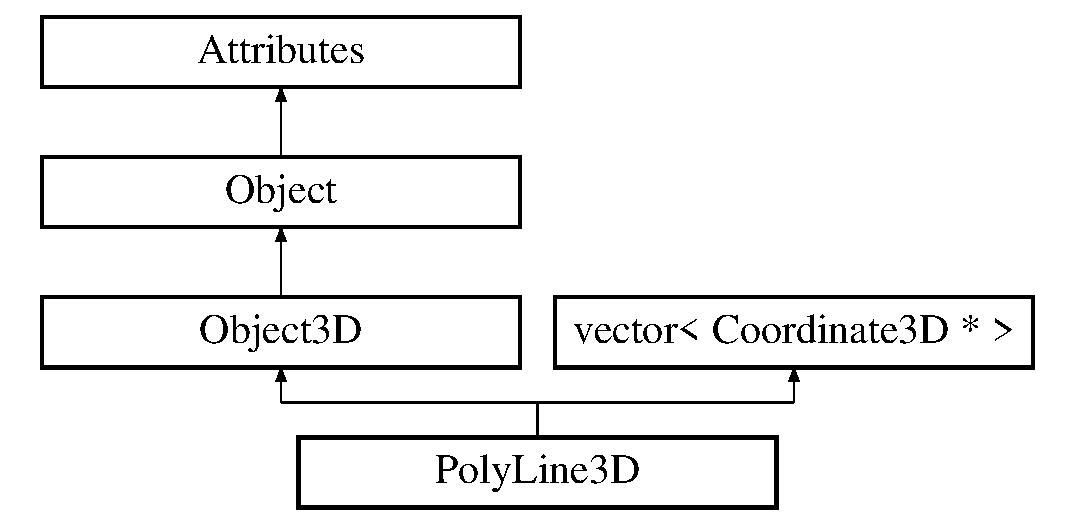
\includegraphics[height=4cm]{classPolyLine3D}
\end{center}
\end{figure}
\subsection*{Public Types}
\begin{CompactItemize}
\item 
enum {\bf Sub\-Types} \{ {\bf Poly\-Line3DType} =   1, 
{\bf Box\-Type} =  2, 
{\bf Polygon\-Type} =  3, 
{\bf Arc\-Box\-Type} =  4, 
{\bf Picture\-Type} =  5
 \}
\end{CompactItemize}
\subsection*{Public Methods}
\begin{CompactItemize}
\item 
{\bf Poly\-Line3D} ()
\item 
{\bf Poly\-Line3D} ({\bf Coordinate3D} $\ast$point1, {\bf Coordinate3D} $\ast$point2)
\item 
{\bf $\sim$Poly\-Line3D} ()
\item 
int {\bf get\-Sub\-Type} ()
\item 
std::pair$<$ double, double $>$ {\bf get\-Depth\-Range} ()
\item 
void {\bf apply\-Matrix} ({\bf Matrix}$<$ double $>$ $\ast$)
\item 
void {\bf render} ({\bf Figure} $\ast$, double x\-Offset, double y\-Offset, double scale, double distance, double min\-Depth, double max\-Depth, int min\-Fig\-Depth=0, int max\-Fig\-Depth=999)
\item 
void {\bf translate} ({\bf Coordinate3D} $\ast$)
\item 
void {\bf write} (std::ostream \&stream) const
\end{CompactItemize}
\subsection*{Protected Methods}
\begin{CompactItemize}
\item 
void {\bf set\-Sub\-Type} ({\bf Sub\-Types} {\bf sub\-Type})
\end{CompactItemize}
\subsection*{Private Attributes}
\begin{CompactItemize}
\item 
{\bf Sub\-Types} {\bf sub\-Type}
\end{CompactItemize}


\subsection{Member Enumeration Documentation}
\index{PolyLine3D@{Poly\-Line3D}!SubTypes@{SubTypes}}
\index{SubTypes@{SubTypes}!PolyLine3D@{Poly\-Line3D}}
\subsubsection{\setlength{\rightskip}{0pt plus 5cm}enum Poly\-Line3D::Sub\-Types}\label{classPolyLine3D_s5}


Enumeration of polyline types. The following types can be used to set the type of a polyline object : \{$\backslash$tt Poly\-Line\-Type, Box\-Type, Polygon\-Type, Picture\-Type\}. Inherited polyline classes will set their appropriate type. \begin{Desc}
\item[Enumeration values: ]\par
\begin{description}
\index{PolyLine3DType@{PolyLine3DType}!PolyLine3D@{PolyLine3D}}\index{PolyLine3D@{PolyLine3D}!PolyLine3DType@{PolyLine3DType}}\item[{\em 
{\em Poly\-Line3DType}\label{classPolyLine3D_s5s0}
}]\index{BoxType@{BoxType}!PolyLine3D@{PolyLine3D}}\index{PolyLine3D@{PolyLine3D}!BoxType@{BoxType}}\item[{\em 
{\em Box\-Type}\label{classPolyLine3D_s5s1}
}]\index{PolygonType@{PolygonType}!PolyLine3D@{PolyLine3D}}\index{PolyLine3D@{PolyLine3D}!PolygonType@{PolygonType}}\item[{\em 
{\em Polygon\-Type}\label{classPolyLine3D_s5s2}
}]\index{ArcBoxType@{ArcBoxType}!PolyLine3D@{PolyLine3D}}\index{PolyLine3D@{PolyLine3D}!ArcBoxType@{ArcBoxType}}\item[{\em 
{\em Arc\-Box\-Type}\label{classPolyLine3D_s5s3}
}]\index{PictureType@{PictureType}!PolyLine3D@{PolyLine3D}}\index{PolyLine3D@{PolyLine3D}!PictureType@{PictureType}}\item[{\em 
{\em Picture\-Type}\label{classPolyLine3D_s5s4}
}]\end{description}
\end{Desc}



\subsection{Constructor \& Destructor Documentation}
\index{PolyLine3D@{Poly\-Line3D}!PolyLine3D@{PolyLine3D}}
\index{PolyLine3D@{PolyLine3D}!PolyLine3D@{Poly\-Line3D}}
\subsubsection{\setlength{\rightskip}{0pt plus 5cm}Poly\-Line3D::Poly\-Line3D ()}\label{classPolyLine3D_a0}


Constructor. Constructs a polyline object \index{PolyLine3D@{Poly\-Line3D}!PolyLine3D@{PolyLine3D}}
\index{PolyLine3D@{PolyLine3D}!PolyLine3D@{Poly\-Line3D}}
\subsubsection{\setlength{\rightskip}{0pt plus 5cm}Poly\-Line3D::Poly\-Line3D ({\bf Coordinate3D} $\ast$ {\em point1}, {\bf Coordinate3D} $\ast$ {\em point2})}\label{classPolyLine3D_a1}


Constructor. Constructs a polyline object with 2 points \begin{Desc}
\item[Parameters: ]\par
\begin{description}
\item[{\em 
point1}]- Instance of {\bf Coordinate3D} {\rm (p.\,\pageref{classCoordinate3D})}. {\bf Coordinate3D} {\rm (p.\,\pageref{classCoordinate3D})} of the first point \item[{\em 
point2}]- Instance of {\bf Coordinate3D} {\rm (p.\,\pageref{classCoordinate3D})}. {\bf Coordinate3D} {\rm (p.\,\pageref{classCoordinate3D})} of the second point \end{description}
\end{Desc}
\index{PolyLine3D@{Poly\-Line3D}!~PolyLine3D@{$\sim$PolyLine3D}}
\index{~PolyLine3D@{$\sim$PolyLine3D}!PolyLine3D@{Poly\-Line3D}}
\subsubsection{\setlength{\rightskip}{0pt plus 5cm}Poly\-Line3D::$\sim$Poly\-Line3D ()}\label{classPolyLine3D_a2}


Destructor. Destructs a polyline object 

\subsection{Member Function Documentation}
\index{PolyLine3D@{Poly\-Line3D}!applyMatrix@{applyMatrix}}
\index{applyMatrix@{applyMatrix}!PolyLine3D@{Poly\-Line3D}}
\subsubsection{\setlength{\rightskip}{0pt plus 5cm}void Poly\-Line3D::apply\-Matrix ({\bf Matrix}$<$ double $>$ $\ast$)\hspace{0.3cm}{\tt  [virtual]}}\label{classPolyLine3D_a5}




Implements {\bf Object3D} {\rm (p.\,\pageref{classObject3D_a2})}.\index{PolyLine3D@{Poly\-Line3D}!getDepthRange@{getDepthRange}}
\index{getDepthRange@{getDepthRange}!PolyLine3D@{Poly\-Line3D}}
\subsubsection{\setlength{\rightskip}{0pt plus 5cm}std::pair$<$ double, double $>$ Poly\-Line3D::get\-Depth\-Range ()\hspace{0.3cm}{\tt  [virtual]}}\label{classPolyLine3D_a4}




Implements {\bf Object3D} {\rm (p.\,\pageref{classObject3D_a0})}.\index{PolyLine3D@{Poly\-Line3D}!getSubType@{getSubType}}
\index{getSubType@{getSubType}!PolyLine3D@{Poly\-Line3D}}
\subsubsection{\setlength{\rightskip}{0pt plus 5cm}int Poly\-Line3D::get\-Sub\-Type ()\hspace{0.3cm}{\tt  [inline]}}\label{classPolyLine3D_a3}


Returns the polyline sub type \begin{Desc}
\item[Returns: ]\par
Instance of {\bf Sub\-Types} {\rm (p.\,\pageref{classPolyLine3D_s5})} \end{Desc}
\index{PolyLine3D@{Poly\-Line3D}!render@{render}}
\index{render@{render}!PolyLine3D@{Poly\-Line3D}}
\subsubsection{\setlength{\rightskip}{0pt plus 5cm}void Poly\-Line3D::render ({\bf Figure} $\ast$, double {\em x\-Offset}, double {\em y\-Offset}, double {\em scale}, double {\em distance}, double {\em min\-Depth}, double {\em max\-Depth}, int {\em min\-Fig\-Depth} = 0, int {\em max\-Fig\-Depth} = 999)\hspace{0.3cm}{\tt  [virtual]}}\label{classPolyLine3D_a6}




Implements {\bf Object3D} {\rm (p.\,\pageref{classObject3D_a1})}.\index{PolyLine3D@{Poly\-Line3D}!setSubType@{setSubType}}
\index{setSubType@{setSubType}!PolyLine3D@{Poly\-Line3D}}
\subsubsection{\setlength{\rightskip}{0pt plus 5cm}void Poly\-Line3D::set\-Sub\-Type ({\bf Sub\-Types} {\em sub\-Type})\hspace{0.3cm}{\tt  [inline, protected]}}\label{classPolyLine3D_b0}


Set the sub type \begin{Desc}
\item[Parameters: ]\par
\begin{description}
\item[{\em 
sub\-Type}]{\bf Sub\-Types} {\rm (p.\,\pageref{classPolyLine3D_s5})} \end{description}
\end{Desc}
\begin{Desc}
\item[Returns: ]\par
void \end{Desc}
\index{PolyLine3D@{Poly\-Line3D}!translate@{translate}}
\index{translate@{translate}!PolyLine3D@{Poly\-Line3D}}
\subsubsection{\setlength{\rightskip}{0pt plus 5cm}void Poly\-Line3D::translate ({\bf Coordinate3D} $\ast$)\hspace{0.3cm}{\tt  [virtual]}}\label{classPolyLine3D_a7}




Implements {\bf Object3D} {\rm (p.\,\pageref{classObject3D_a3})}.\index{PolyLine3D@{Poly\-Line3D}!write@{write}}
\index{write@{write}!PolyLine3D@{Poly\-Line3D}}
\subsubsection{\setlength{\rightskip}{0pt plus 5cm}void Poly\-Line3D::write (std::ostream \& {\em stream}) const\hspace{0.3cm}{\tt  [virtual]}}\label{classPolyLine3D_a8}


Write the polyline object to a given outstream. \begin{Desc}
\item[Parameters: ]\par
\begin{description}
\item[{\em 
stream}]output stream \end{description}
\end{Desc}
\begin{Desc}
\item[Returns: ]\par
void \end{Desc}


Reimplemented from {\bf Object} {\rm (p.\,\pageref{classObject_a3})}.

\subsection{Member Data Documentation}
\index{PolyLine3D@{Poly\-Line3D}!subType@{subType}}
\index{subType@{subType}!PolyLine3D@{Poly\-Line3D}}
\subsubsection{\setlength{\rightskip}{0pt plus 5cm}{\bf Sub\-Types} Poly\-Line3D::sub\-Type\hspace{0.3cm}{\tt  [private]}}\label{classPolyLine3D_o0}




The documentation for this class was generated from the following files:\begin{CompactItemize}
\item 
{\bf polyline3d.h}\item 
{\bf polyline3d.cpp}\end{CompactItemize}
